\subsection{Affine Varieties}


\begin{exercise}{1}
Sketch the following affine varieties in $\R^2$:
\begin{enumerate}
    \item $\bV(x^2 + 4y^2 + 2x - 16y + 1)$.
    \item $\bV(x^2 - y^2)$.
    \item $\bV(2x+y-1, 3x - y + 2)$.
\end{enumerate}
In each case, does the variety have the dimension you would intuitively expect it to have.
\end{exercise}
\begin{proof}
    \begin{enumerate}
        \item This will turn out to be an ellipse.
        \begin{figure}[H]
            \centering
            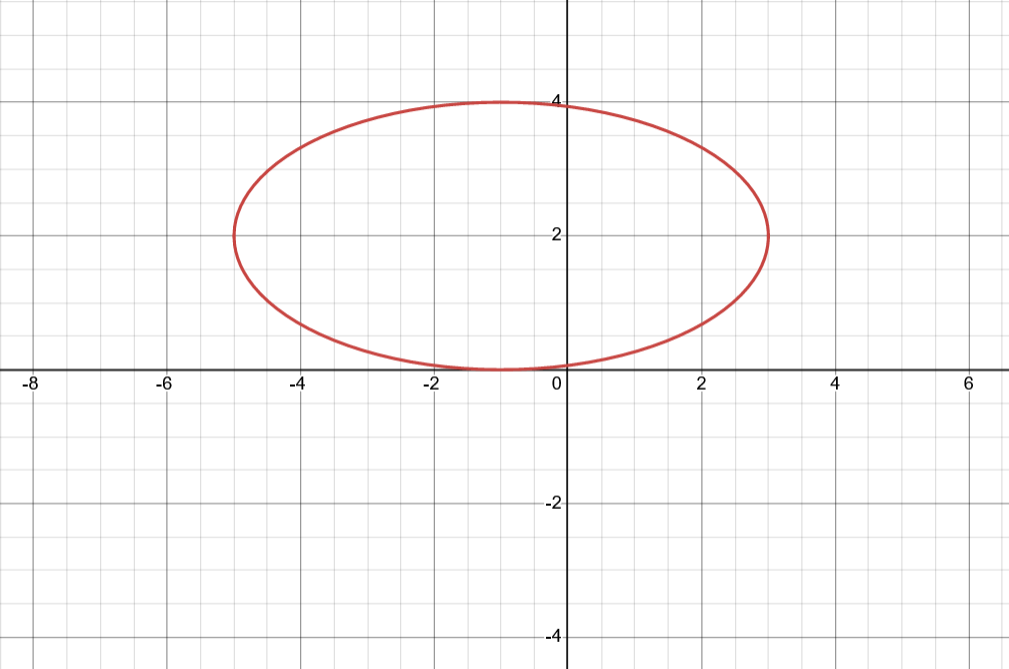
\includegraphics[width=0.5\linewidth]{cox-little-oshea/assets/sec1-2-ex1a.png}
     \caption{Graph of $\bV(x^2 + 4y^2 + 2x - 16y + 1)$}
     \label{fig:sec1-2-ex1a}
        \end{figure}
        I would expect a dimension of $1$, which the figure does seem to indicate.
        \item This is a union of the lines $x=\pm y$.
        \begin{figure}[H]
            \centering
            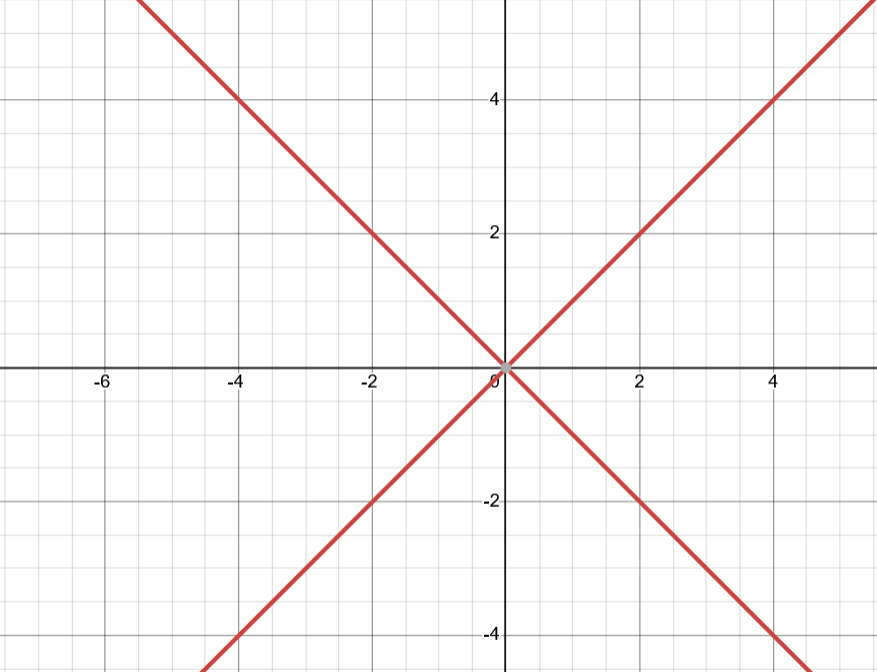
\includegraphics[width=0.5\linewidth]{cox-little-oshea/assets/sec1-2-ex1b.png}
            \caption{Graph of $\bV(x^2 - y^2)$}
            \label{fig:sec1-2-ex1b}
        \end{figure}
        I would expect a dimension of $1$, which the figure does seem to indicate except perhaps in the origin.
        \item Solving the system
        $$\left\{\begin{array}{l}
        2x + y - 1 = 0\\
        3x - y + 2 = 0,
        \end{array}\right.$$
        we get as only solution $\left(-\frac{1}{5},\frac{7}{5}\right)$. The variety will just be a single point.
        \begin{figure}[H]
            \centering
            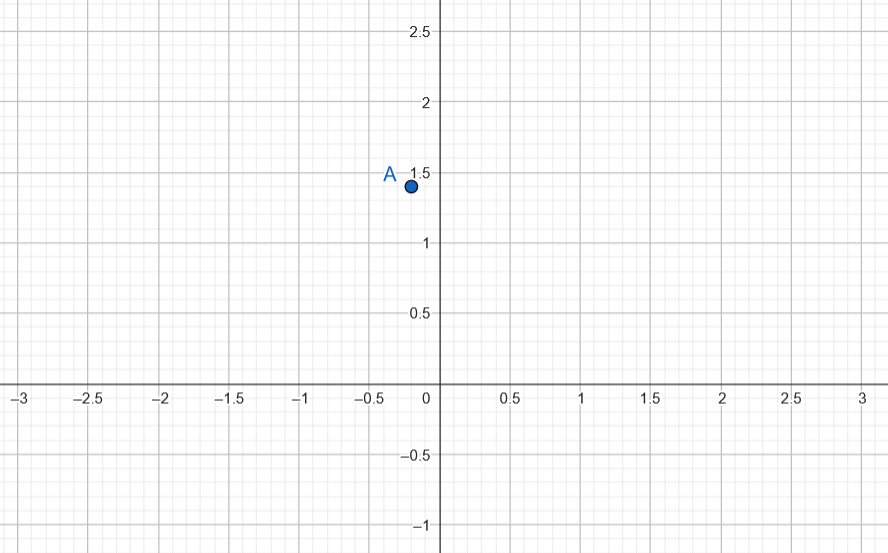
\includegraphics[width=0.5\linewidth]{cox-little-oshea/assets/sec1-2-ex1c.png}
            \caption{Graph of $\bV(2x+y-1, 3x - y + 2)$}
            \label{fig:sec1-2-ex1c}
        \end{figure}
        I would expect a dimension of $0$, which a single point does have.
    \end{enumerate}
\end{proof}

\begin{exercise}{2}
In $\R^2$, sketch $\bV(y^2-x(x-1)(x-2))$. Hint: For which $x$'s is it possible to solve for $y$? How many $y$'s correspond to each $x$? What symmetry does the curve have?
\end{exercise}
\begin{proof}
I will use a graphing calculator for this exercise, but still will answer the hint questions. If we solve for $y$, we obtain $y=\sqrt{x(x-1)(x-2)}$, so that we can solve for $y$, whenever $x(x-1)(x-2)\geq 0$. We require that either all of $x, x-1$ and $x-2$ are non-negative, or exactly two of them are negative. All of them are non-negative whenever $x\geq 2$ and two of them are negative whenever $0<x<1$. For these values of $x$ we have two values of $y$ (positive and negative), and hence we obtain symmetry with respect to the $x$-axis.
 \begin{figure}[H]
     \centering
     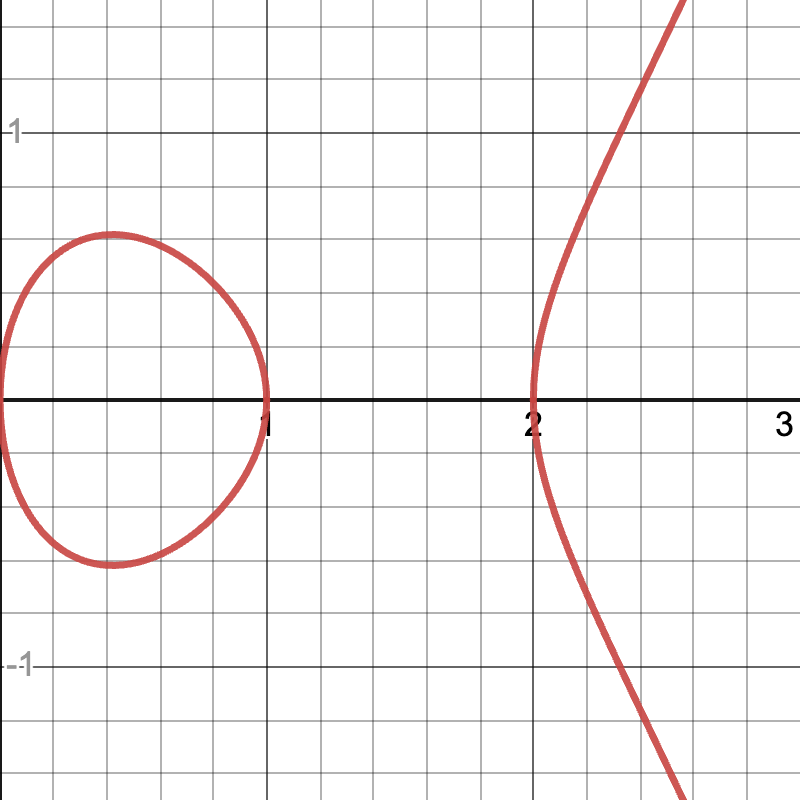
\includegraphics[width=.5\textwidth]{cox-little-oshea/assets/sec1-2-ex2.png}
     \caption{Graph of $\bV(y^2-x(x-1)(x-2))$}
     \label{fig:sec1-2-ex2}
 \end{figure}
\end{proof}

\begin{exercise}{3}
In the plane $\R^2$, draw a picture to illustrate $\bV(x^2+y^2-4)\cap\bV(xy-1)=\bV(x^2+y^2-4,xy-1)$, and determine the points of intersection. Note that this is a special case of lemma 2.
\end{exercise}
\begin{proof}
 \begin{figure}[H]
     \centering
     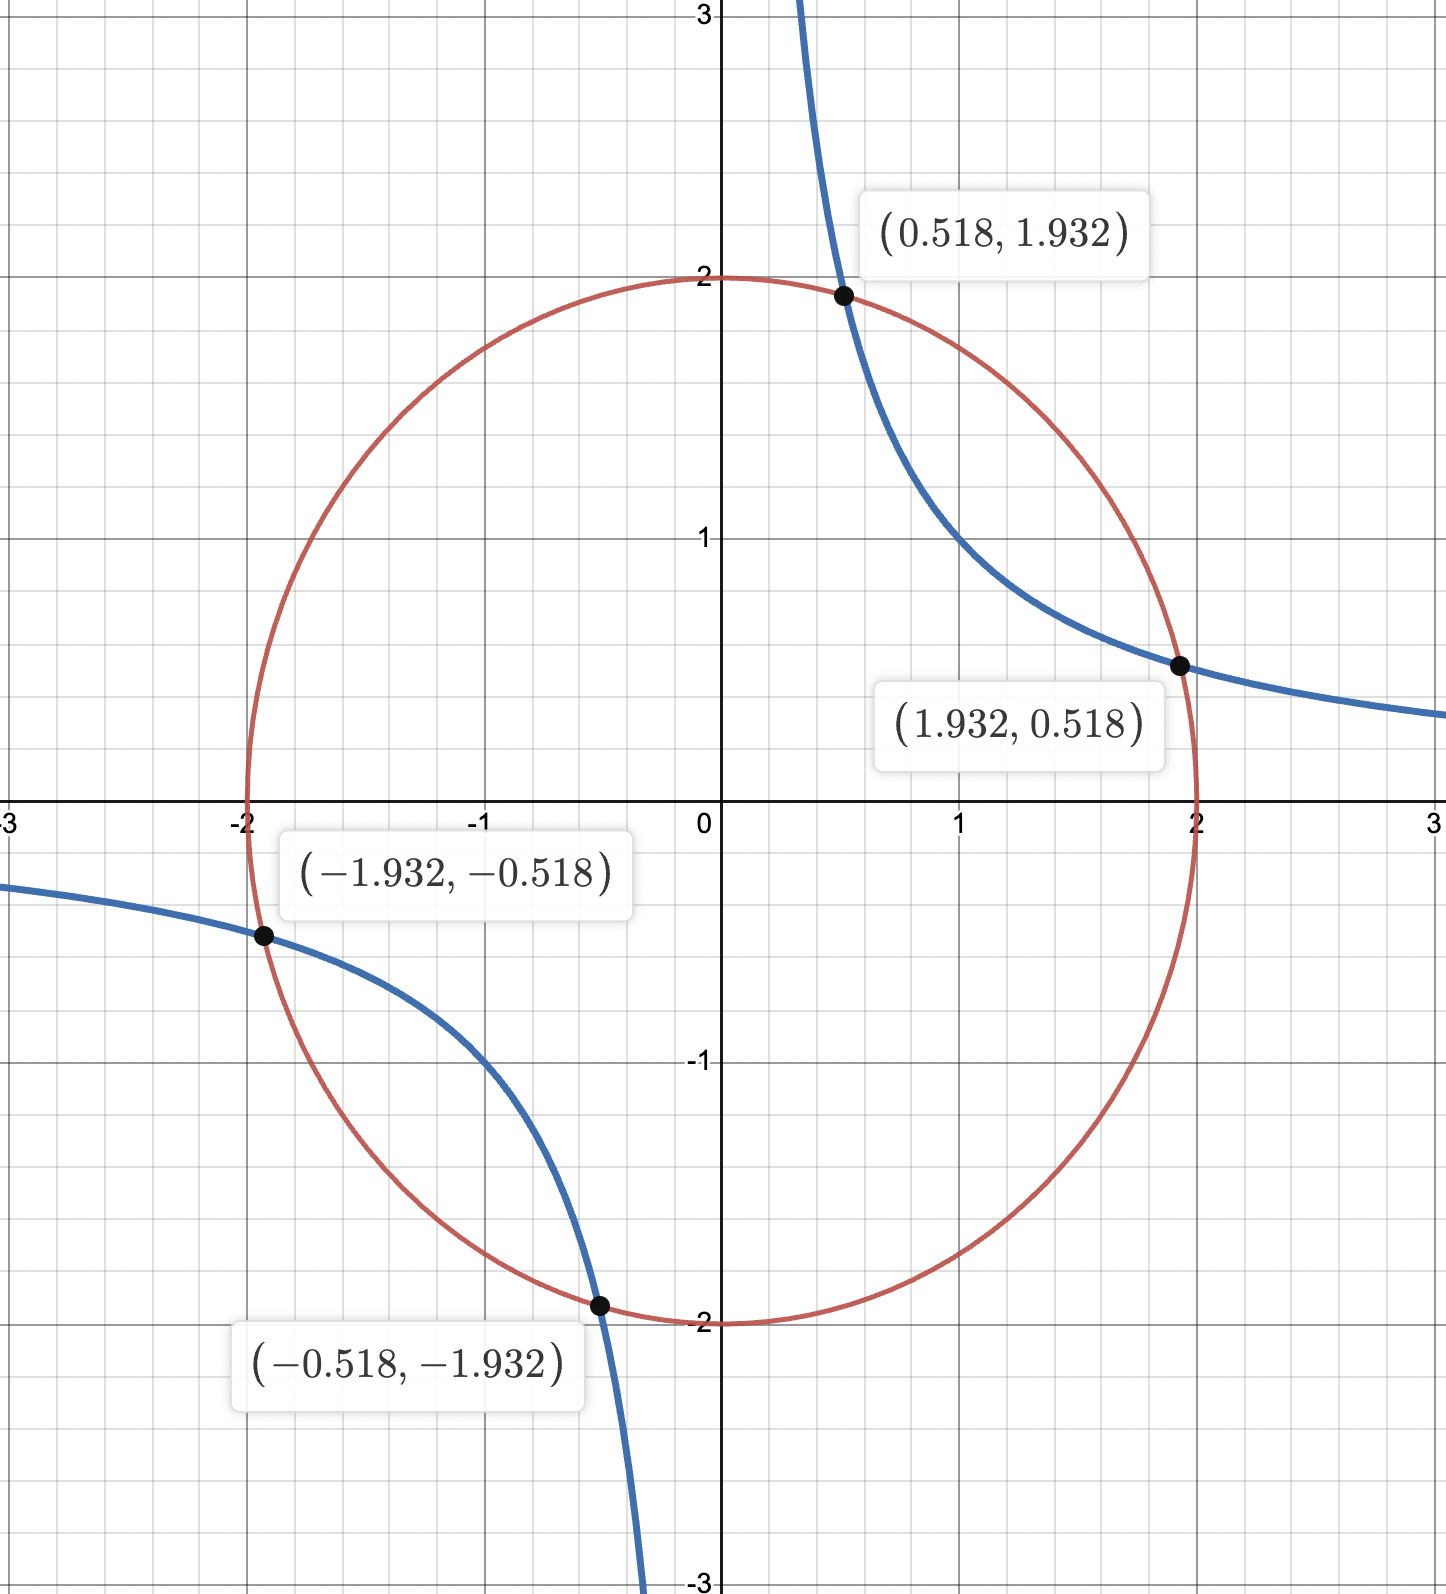
\includegraphics[width=.5\textwidth]{cox-little-oshea/assets/sec1-2-ex3.png}
     \caption{Graph of $\bV(x^2+y^2-4), \bV(xy-1)$, and its intersection points}
     \label{fig:sec1-2-ex3}
 \end{figure}
\end{proof}

\begin{exercise}{4}
Sketch the following affine varieties in $\R^3$:
\begin{enumerate}
    \item $\bV(x^2 + y^2 + z^2 - 1)$.
    \item $\bV(x^2 + y^2 - 1)$.
    \item $\bV(x+2, y-1.5, z)$.
    \item $\bV(xz^2 - xy)$.
    \item $\bV(x^4 - zx, x^2 - yx)$.
    \item $\bV(x^2 + y^2 + z^2 - 1, x^2 + y^2 + (z-1)^2 - 1)$.
\end{enumerate}
In each case, does the variety have the dimension you would intuitively expect it to have.
\end{exercise}
\begin{proof}
    \begin{enumerate}
        \item This is a sphere of radius $1$.
        \begin{figure}[H]
            \centering
            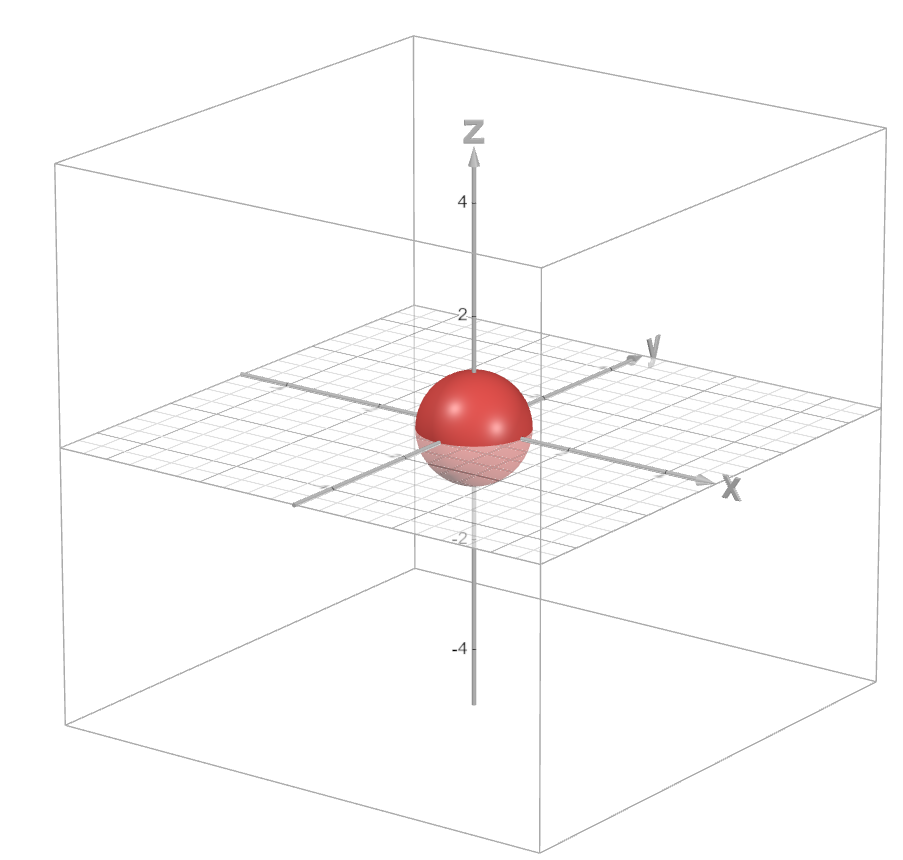
\includegraphics[width=0.5\linewidth]{cox-little-oshea/assets/sec1-2-ex4a.png}
            \caption{Graph of $\bV(x^2+y^2+z^2-1)$}
            \label{fig:sec1-2-ex4a}
        \end{figure}
        I would expect it to have dimension $2$, which is true.
        \item This is a cylinder of radius $1$.
        \begin{figure}[H]
            \centering
            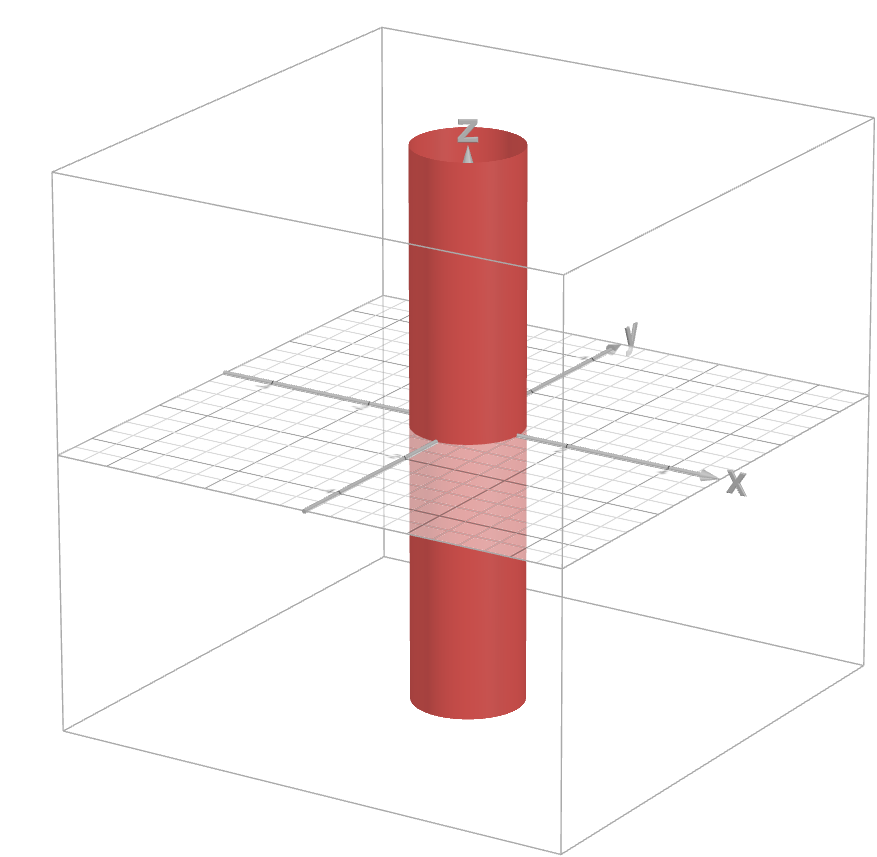
\includegraphics[width=0.5\linewidth]{cox-little-oshea/assets/sec1-2-ex4b.png}
            \caption{Graph of $\bV(x^2+y^2-1)$}
            \label{fig:sec1-2-ex4b}
        \end{figure}
        I would expect this to have dimension $2$, and it does.
        \item This is simply a point
        \begin{figure}[H]
            \centering
            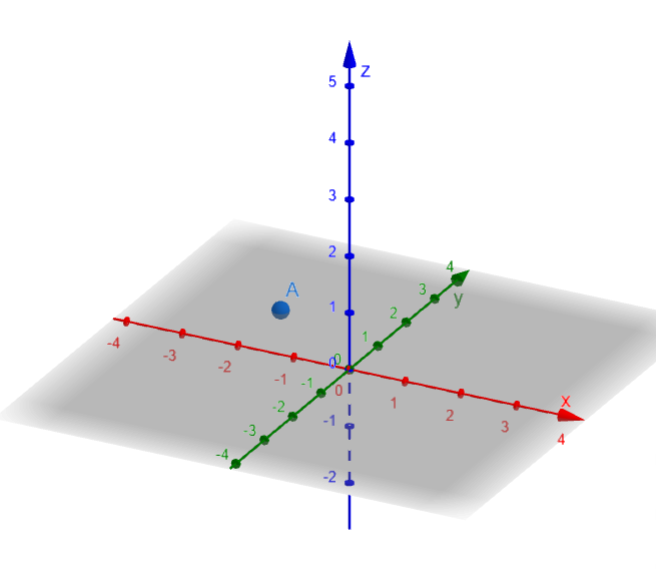
\includegraphics[width=0.5\linewidth]{cox-little-oshea/assets/sec1-2-ex4c.png}
            \caption{Graph of $\bV(x+2, y-1.5, z)$}
            \label{fig:sec1-2-ex4c}
        \end{figure}
        I would expect this to have dimension $0$ and it does.
        \item This is $\bV(x)\cup \bV(z^2 - y)$. 
        \begin{figure}[H]
            \centering
            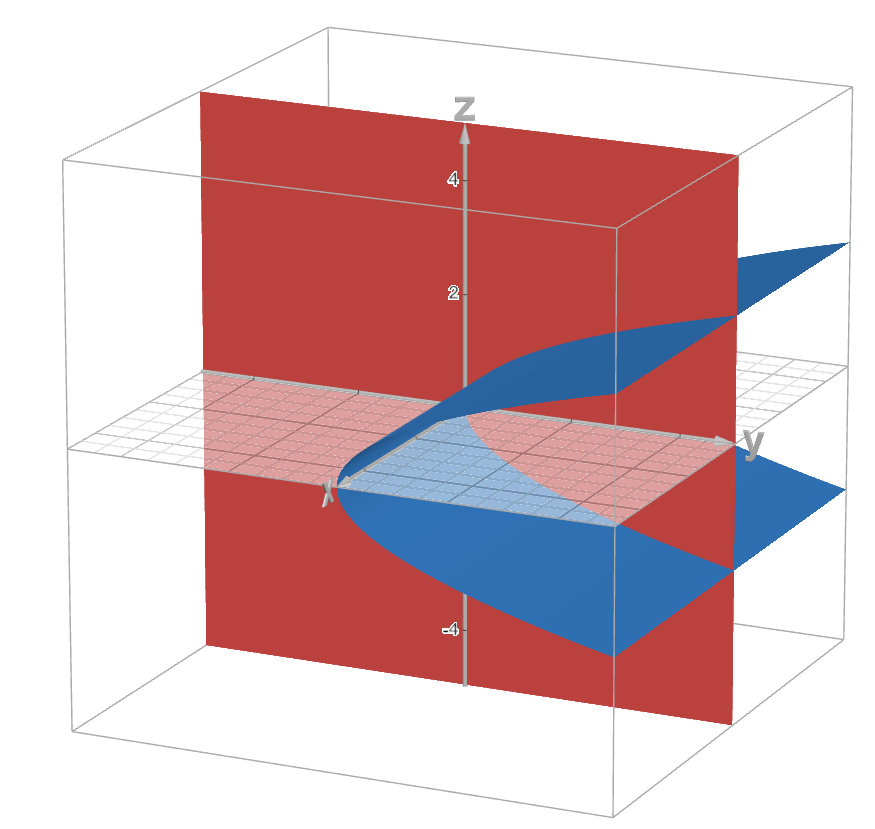
\includegraphics[width=0.5\linewidth]{cox-little-oshea/assets/sec1-2-ex4d.png}
            \caption{Graph of $\bV(xz^2 - xy)$}
            \label{fig:sec1-2-ex4d}
        \end{figure}
        We expect this to have dimension $2$, and it kind of does except in the intersection points perhaps.
        \item We have to solve
        $$x(x^3 - z) = 0,~x(x^2 - y) = 0.$$
        Clearly the equation $x=0$ is a solution. Now assume that $x\neq 0$, then we get the solution curve given by $(t,t^2,t^3)$.
        \begin{figure}
            \centering
            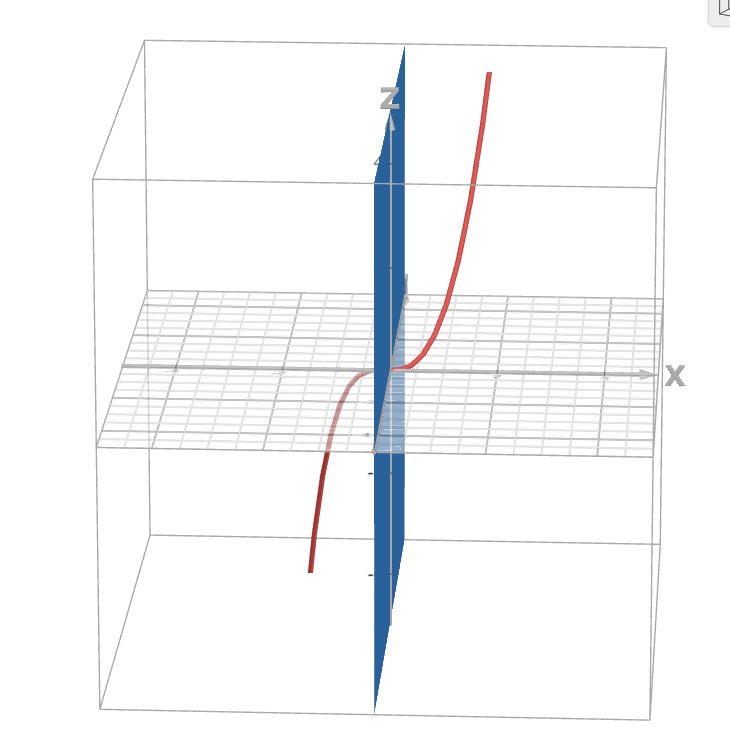
\includegraphics[width=0.5\linewidth]{cox-little-oshea/assets/sec1-2-ex4e.png}
            \caption{Graph of $\bV(x^4 - zx, x^3 - yx)$}
            \label{fig:sec1-2-ex4e}
        \end{figure}
        We expect this to have dimension $1$, but a lot of the points on the variety have dimension $2$.
        \item We get that
        $$z^2 = 1 - x^2 - y^2 = (z-1)^2.$$
        Clearly this implies $z=z-1$ or $z=1-z$. The former can never happen, and the latter implies $z = \frac{1}{2}$. We get the equation
        $$x^2 + y^2 = \frac{3}{4}.$$
        This is a cylinder.
        \begin{figure}
            \centering
            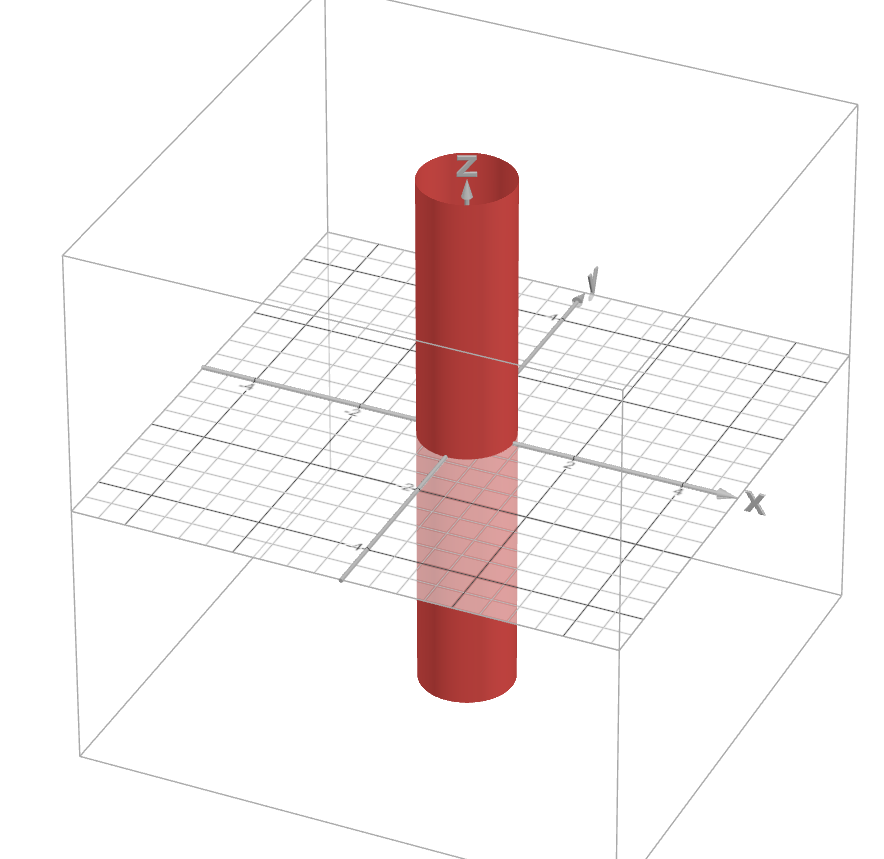
\includegraphics[width=0.5\linewidth]{cox-little-oshea/assets/sec1-2-ex4f.png}
            \caption{Graph of $\bV(x^2 + y^2 + z^2 - 1, x^2 + y^2 + (z-1)^2 - 1)$}
            \label{fig:sec1-2-ex4f}
        \end{figure}
        We expect this to have dimension $1$, but we get a variety of dimension $2$.
    \end{enumerate}
\end{proof}

\begin{exercise}{5}
Use the proof of Lemma $2$ to sketch $\bV( (x-2)(x^2 - y), y(x^2 - y), (z+1)(x^2-y))$ in $\R^3$.
\end{exercise}
\begin{proof}
    We get that this is
    $$\bV(x^2 - y)\cup \bV(x-2, y, z+1).$$
    So it is the union of the variety given by equation $y=x^2$ and the point $(2,0,-1)$.
    \begin{figure}
        \centering
        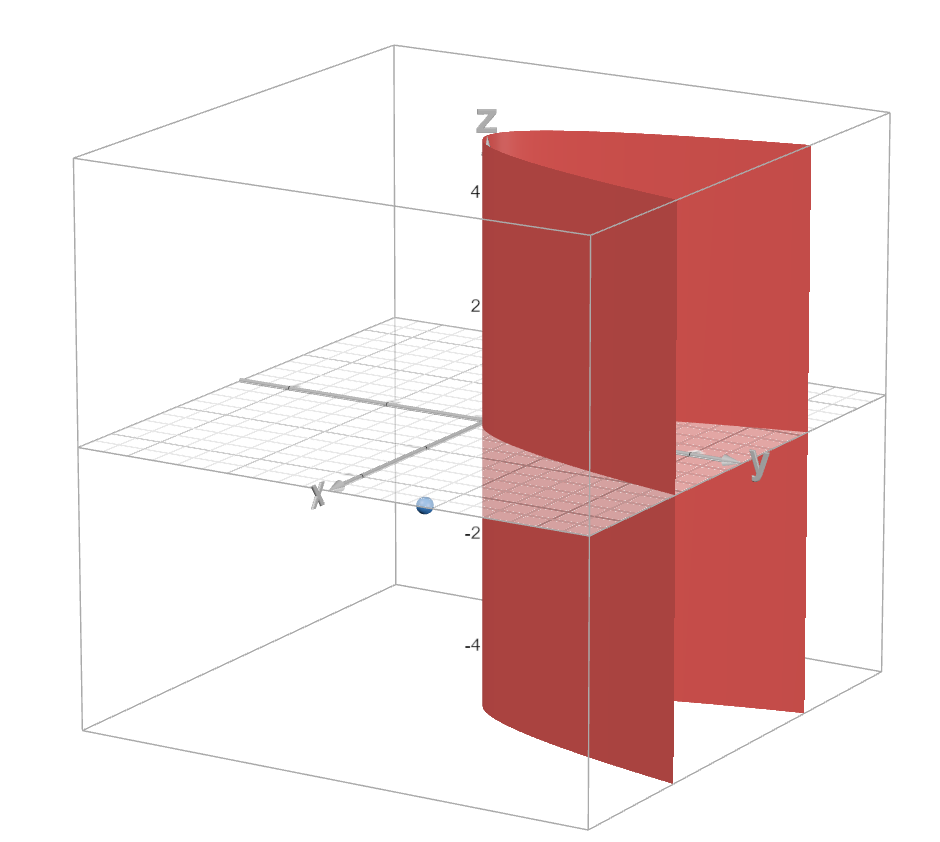
\includegraphics[width=0.5\linewidth]{cox-little-oshea/assets/sec1-2-ex5.png}
            \caption{Graph of $\bV( (x-2)(x^2 - y), y(x^2 - y), (z+1)(x^2-y))$}
            \label{fig:sec1-2-ex5}
    \end{figure}
\end{proof}

\begin{exercise}{6}
Let us show that all finite subsets of $k^n$ are affine varieties.
\begin{enumerate}
    \item Prove that a single point $(a_1,\dots,a_n)\in k^n$ is an affine variety.
    \item Prove that every finite subset of $k^n$ is an affine variety. Hint: Lemma 2 will be useful.
\end{enumerate}
\end{exercise}
\begin{proof}
 \begin{enumerate}
     \item Consider the set of polynomials $f_1,\dots,f_n$ given by $f_i(x_i)=x_i-a_i$. Then certainly $\bV(f_1,\dots,f_n)$ has as variety the point $(a_1,\dots,a_n)\in k^n$, as required.
     \item We have just proven above that any point is an affine variety of a particular set of polynomials, so that for any point in the set we are interested in, say $(a_{i,1},\dots,a_{i,n})$ is a variety $\bV_i$ of a set of polynomials. From Lemma 2, we know that the union of two varieties is a variety, hence, $\cup_{i=1}^{m}\bV_i$ is a variety.
 \end{enumerate}
\end{proof}

\begin{exercise}{7}
One of the prettiest examples from polar coordinates is the four-leaved rose. This curve is defined by the polar equation $r=\sin(2\theta)$. We will show that this curve is an affine variety.
\begin{enumerate}
    \item Using $r^2 = x^2 + y^2$, $x=r\cos(\theta)$ and $y=r\sin(\theta)$, show that the four-leaved rose is contained in the affine variety $\bV( (x^2 + y^2)^3 - 4x^2 y^2)$.
    \item Now argue carefully that $\bV((x^2 + y^2)^3 - 4x^2 y^2)$ is contained in the four-leaved rose. This is trickier than it seems since $r$ can be negative in $r=\sin(2\theta)$.
\end{enumerate}
Combining parts (a) and (b), we have proved that the four-leaved rose is the affine variety $\bV((x^2 + y^2)^3 - 4x^2 y^2)$.
\end{exercise}
\begin{proof}
    \begin{enumerate}
        \item We get that
        \begin{eqnarray*}
            (x^2 + y^2)^3 - 4x^2 y^2
            & = & (r^2)^3 - 4(r\cos\theta)^2 (r\sin\theta)^2\\
            & = & r^6 - 4r^4 \cos^2\theta \sin^2\theta\\
            & = & r^6 - r^4 \sin^2(2\theta)\\
            & = & r^4(r^2 - \sin^2(2\theta))\\
            & = & r^4(r-\sin(2\theta))(r+\sin(2\theta))\\
            & = & 0.
        \end{eqnarray*}
        \item Take a point $(x,y)$ with $(x^2 + y^2)^3 = 4x^2y^2$. We can find some angle $\theta$ such that $(x,y) = (r\cos\theta, r\sin\theta)$. Then,
        \begin{eqnarray*}
            0
            & = & (x^2 + y^2)^3 - 4x^2 y^2\\
            & = & (r^2\cos^2\theta + r^2\sin^2\theta)^3 - 4(r\cos\theta)^2 (r\sin\theta)^2\\
            & = & r^6 - 4r^4 \cos^2\theta \sin^2\theta\\
            & = & r^6 - r^4 \sin^2(2\theta)\\
            & = & r^4 (r^2 - \sin^2(2\theta)).
        \end{eqnarray*}
        There are a few possibilities on $r$:
        \begin{itemize}
            \item If $r=0$, then $(x,y) = (0,0)$, but then we can choose $r=0$ and $\theta = 0$ and then the equation $r=\sin(2\theta)$ will be satisfied.
            \item If $r\neq 0$, then $|r| = |\sin(2\theta)|$. If $r = \sin(2\theta)$, the result has been shown. In the other case, we have $r=-\sin(2\theta)$. In that case, we notice that
            \begin{eqnarray*}
                -r
                & = & \sin(2\theta)\\
                & = & \sin(2\theta + 2\pi)\\
                & = & \sin(2(\theta + \pi)),
            \end{eqnarray*}
            and $(x,y) = (-r\cos(\pi + \theta), -r\sin(\pi + \theta))$, and thus $(x,y)$ also has $r$ and $\theta$ such that $r=\sin(2\theta)$, namely $-r$ and $\pi+\theta$.
        \end{itemize}
    \end{enumerate}
\end{proof}

\begin{exercise}{8}
It can take some work to show that something is not an affine variety. For example, consider the set $X=\{(x,x)\mid x\in\R, x\neq 1\}\subseteq\R^2$, which is the straight line $x=y$ with the point $(1,1)$ removed. To show that $X$ is not an affine variety, suppose that $X=\bV(f_1,\dots,f_s)$. Then each $f_i$ vanishes on $X$, and if we can show that $f_i$ also vanishes at $(1,1)$, we will get the desired contradiction. Thus, here is what you are to prove: if $f\in\R[x,y]$ vanishes on $X$, then $f(1,1)=0$. Hint: let $g(t)=f(t,t)$, which is a polynomial $\R[t]$. Now apply the proof of Proposition 5 of Section 1.
\end{exercise}
\begin{proof}
 If $f_i$ vanishes on $X$, then $f_i$ has infinitely many roots. But we know that a polynomial with infinitely many roots must be the zero polynomial. Hence, $f_i=0$ and $f_i(1,1)=0$, as required.
\end{proof}

\begin{exercise}{9}
Let $R = \{(x,y)\in \mathbb{R}^2~\vert~y>0\}$ be the upper half plane. Prove that $R$ is not an affine variety.
\end{exercise}
\begin{proof}
    Assume that $R = \bV(f_1,...,f_s)$. Then each $f_i$ vanishes on $R$. Let $f\in \mathbb{R}[x,y]$ be any polynomial vanishing on $R$, then take $g(t) = f(a+t,t)$. We see that $g$ is a polynomial with infinitely many zeroes. Since $\mathbb{R}$ is an infinite field, we must then have $g = 0$. Thus for all $a,t\in \mathbb{R}$, we must have $f(a+t,t) = 0$. Thus $f = 0$ on $R$. In particular, we see that $f_1 = ... = f_s = 0$. Thus
    $$R = \bV(f_1,...,f_s) = \mathbb{R}^2,$$
    which is a contradiction.
\end{proof}

\begin{exercise}{10}
Let $\mathbb{Z}^n\subseteq \mathbb{C}^n$ consists of those points with integer coordinates. Prove that $\mathbb{Z}^n$ is not an affine variety.    
\end{exercise}
\begin{proof}
    Write $\mathbb{Z}^n = \bV(f_1,...,f_s)$. For every $i$ then, we see that $f_i$ vanishes at all points of $\mathbb{Z}^n$. By exercise \S $1.6$, we see then that $f_i = 0$. This holds for arbitrary $i$, hence
    $$\mathbb{Z}^n = \bV(0) = \mathbb{C}^n,$$
    a contradiction.
\end{proof}

\begin{exercise}{11}
So far we have discussed varieties of $\R$ or $\C$. It is also possible to consider varieties over the field $\Q$, although the questions here tend to be much harder. For example, let $n$ be a positive integer, and consider the variety $F_n\subseteq\Q^2$ defined by $x^n+y^n=1$. Notice that there are some obvious solutions when $x$ or $y$ is zero. We call these trivial solutions. An interesting question is whether or not there are nontrivial solutions.
\begin{enumerate}
    \item Show that $F_n$ has two trivial solutions if $n$ is odd and four trivial solutions if $n$ is even.
    \item Show that $F_n$ has a nontrivial solution for some $n\geq 3$ if and only if Fermat's Last Theorem were false.
\end{enumerate}
Fermat's Last Theorem states that, for $n\geq 3$, the equation $x^n+y^n=z^n$ has no solutions where $x,y$ and $z$ are nonzero integers. The general case of this conjecture was proved by Andrew Wiles in 1994 using some very sophisticated number theory. The proof is extremely difficult.
\end{exercise}
\begin{proof}
    \begin{enumerate}
        \item Odd $n$. The trivial solutions are characterised by $x=0$ or $y=0$. Without loss of generality, suppose $x=0$. Since $n$ is odd, if $y=-1$, then $y^n=-1$ so that the equation is not satisfied. Hence $y$ must be equal to 1. We can conclude the same for $x$ if $y=0$. So that there are 2 trivial solutions in total.

        Even $n$. We can follow the same approach as above. Simply notice that if $x=0$ and $y=-1$, we have that $y^n=1$ so that  $y=\pm1$ are valid solutions. We can reason the same for $x$ when $y=0$ so that we obtain 4 trivial solutions.
        \item ($\Rightarrow$) Suppose $F_n$ has a nontrivial solution. Then there exist $x/p,y/q\in\Q$ and $x,p,y,q\in\Z$ such that $(x/p)^n+(y/q)^n=1$. Let $k=\lcm(p,q)$, so that $k\in\Z$. Then $(xq)^n+(yp)^n=k^n$. Since $n\geq 3$ and $xq,yp,k\in\Z$ the equation from the previous sentence would imply that Fermat's Last Theorem is false.

        ($\Leftarrow$) Suppose Fermat's Last Theorem is false. Then there exist $x,y,z\in\Z$ such that $x^n+y^n=z^n$ for some $n\geq 3$. However, this implies $(x/z)^n+(y/z)^n=1$. That is, $p^n+q^n=1$, where $p,q\in\Q$, as required.
    \end{enumerate}
\end{proof}

\begin{exercise}{12}
    Find a Lagrange multipliers problem in a calculus book and write down the corresponding system of equations. Be sure to use an example where one wants to find the minimum or maximum of a polynomial function subject to a polynomial constraint. This way the equations define an affine variety, and try to find a problem that leads to complicated equations. Later we will use the Gr\"obner basis methods to solve these equations.
\end{exercise}
\begin{proof}
    Consider the following problem:\\

    The sum of the lengths of $12$ edges of a rectangular block is $a$; the sum of the area of the $6$ faces is $a^2/25$. Calculate the lengths of the edges when the excess of the volume of the block over that of a cube, whose edges is equal to the least edge of the block, is greatest.\\

    Let the edges of the block be $e\leq f\leq g$. We need to maximize
    $$efg - e^3,$$
    with respect to the constraints
    $$4(e+f+g) = a,~~2(ef + eg + fg) = \frac{a^2}{25}.$$
    We get the following equations:
    $$fg - 3e^2 = 4\lambda + 2\lambda' (f+g),$$
    $$eg = 4\lambda + 2\lambda' (e+g),$$
    $$ef = 4\lambda + 2\lambda' (e+f).$$
\end{proof}

\begin{exercise}{13}
Consider a robot arm in $\mathbb{R}^2$ that consists of three arms of lengths $3$, $2$, and $1$, respectively. The arm of length $3$ is anchored at the origin, the arm of length $2$ is attached to the free end of the arm of length $3$, and the arm of length $1$ is attached to the free end of the arm of length $2$. The ``hand'' of the robot arm is attached to the of the arm of length $1$.
\begin{enumerate}
    \item Draw a picture of the robot arm.
    \item How many variables does it take to determine the ``state'' of the robot arm?
    \item Give the equations for the variety of possible states.
    \item Using the intuitive notion of dimension discussed in this section, guess what dimension of the variety of states should be.
\end{enumerate}
\end{exercise}
\begin{proof}
    \begin{enumerate}
        \item 
\begin{figure}[H]
        \centering
        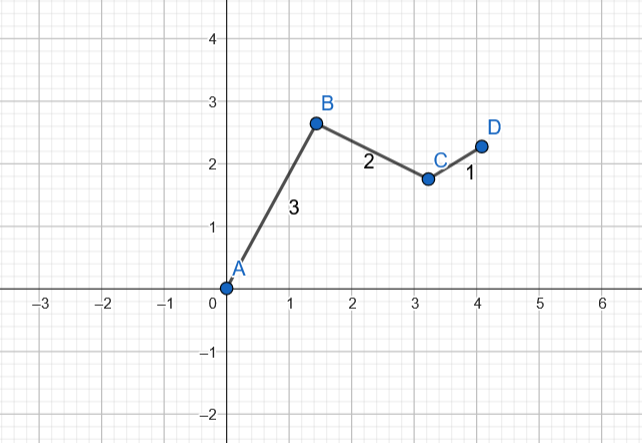
\includegraphics[width=0.5\linewidth]{cox-little-oshea/assets/sec1-2-ex13.png}
        \caption{An example position of the robot arm}
        \label{fig:sec1-2-ex13}
    \end{figure}
    \item It takes $3$ variables: the angle of each arm with the $x$-axis.
    \item To describe the first arm, we have
    $$x^2 + y^2 = 9.$$
    To describe the second arm, we have
    $$(a-x)^2 + (b-y)^2 = 4.$$
    To describe the third arm, we have
    $$(u-a)^2 + (v-b)^2 = 1.$$
    \item There are $3$ equations in (c) with a total of $6$ variables. We expect the dimension to be $6-3 = 3$. This is in line with (b).
\end{enumerate}
\end{proof}

\begin{exercise}{14}
This exercise will study the possible ``hand'' positions of the robot arm described in Exercise $13$.
\begin{enumerate}
    \item If $(u,v)$ is the position of the hand, explain why $u^2 + v^2 \leq 36$.
    \item Suppose we ``lock the joint between the length $3$ and length $2$ arms to form a straight angle, but allow the other joint to move freely. Draw a picture to show that in these configurations, $(u,v)$ can be any point of the annulus $16\leq u^2 + v^2 \leq 36$.
    \item Draw a picture to show that $(u,v)$ can be any point in the disk $u^2 + v^2\leq 36$.
\end{enumerate}
\end{exercise}
\begin{proof}
    \begin{enumerate}
        \item The furthest the hand gets from the origin is when all three arms are on one line. To find how far the hand is, it suffices to add the lengths of the three arms to get $3+2+1 = 6$. Thus $(u,v)$ must always be a distance $6$ or less away from the origin, leading to $u^2 + v^2 \leq 36$.
        \item We get
        \begin{figure}[H]
            \centering
            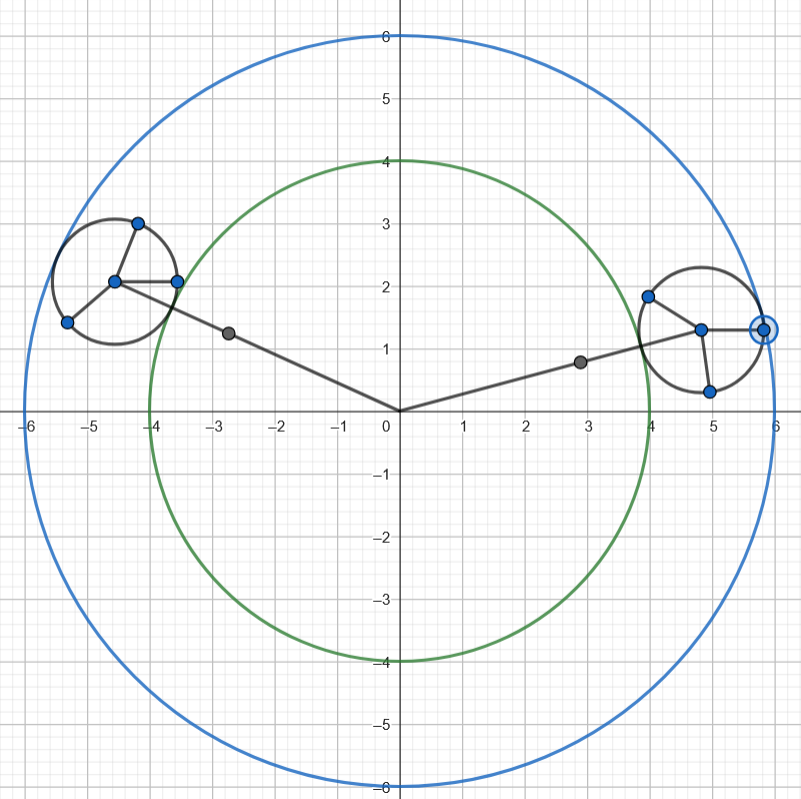
\includegraphics[width=0.5\linewidth]{cox-little-oshea/assets/sec1-2-ex14b.png}
            \caption{Some different configurations of the arm with one joint locked.}
            \label{fig:sec1-2-ex14b}
        \end{figure}
        \item The case $16\leq u^2 + v^2\leq 36$ has already been done in part (b). For $4\leq u^2 + v^2\leq 16$, we fold the length $1$ arm onto the length $2$ arm and lock the joint. We effectively get an arm of length $1$ at the end of an arm of length $3$. 
        \begin{figure}
            \centering
            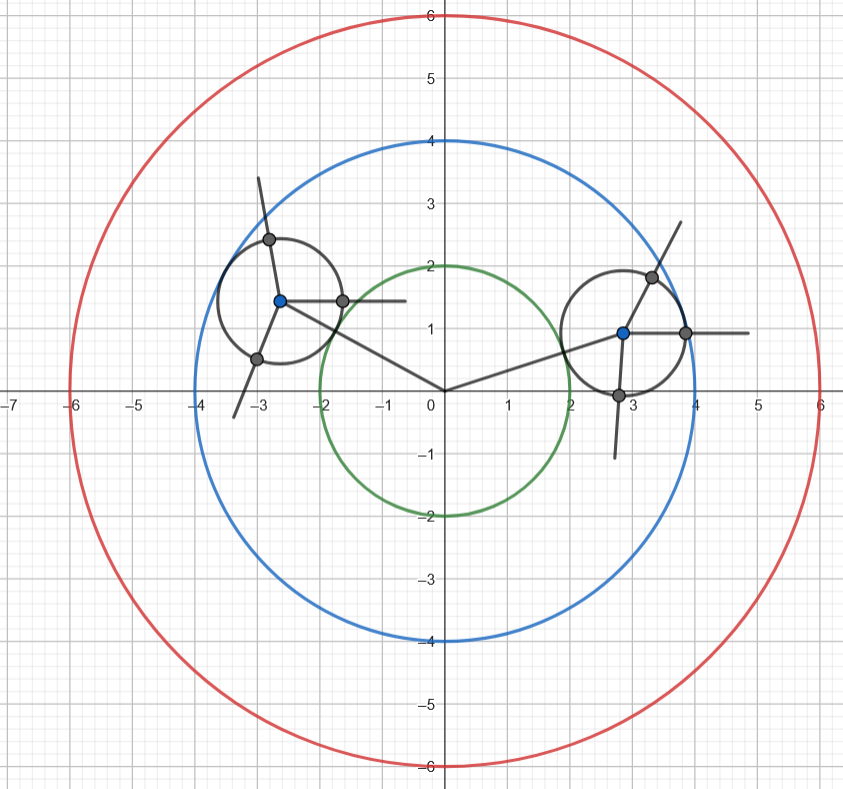
\includegraphics[width=0.5\linewidth]{cox-little-oshea/assets/sec1-2-ex14c.png}
            \caption{Some different configurations of the arm with one joint locked and folded in.}
            \label{fig:sec1-2-ex14c}
        \end{figure}
        For $leq u^2 + v^2\leq 4$, we fold the length $2$ arm onto the length $3$ arm and lock the joint. We effectively get an arm of length $1$ at the end of an arm of length $1$. 
        \begin{figure}
            \centering
            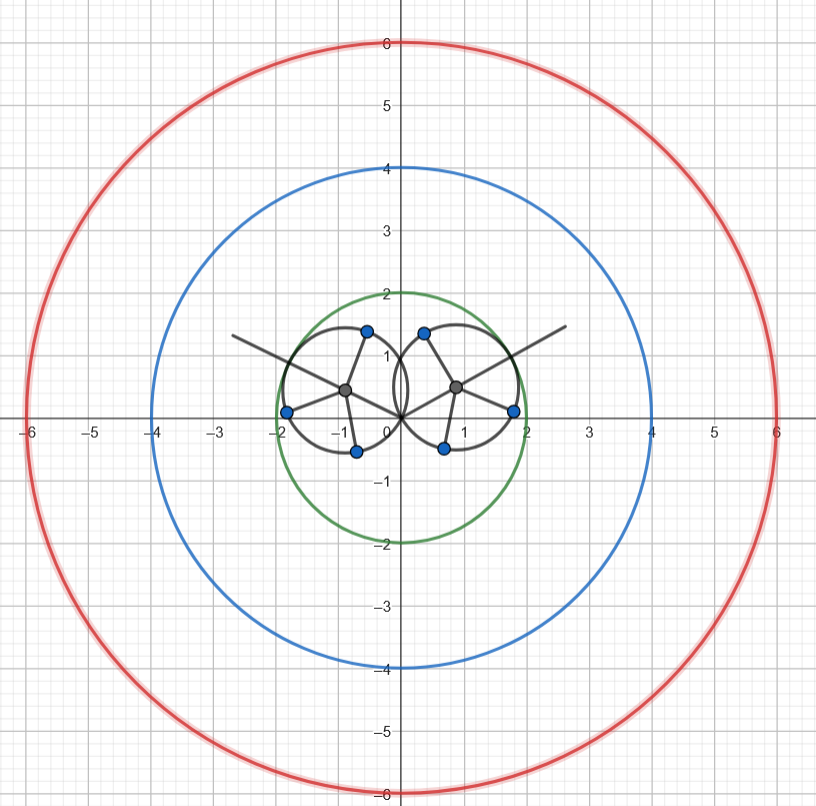
\includegraphics[width=0.5\linewidth]{cox-little-oshea//assets/sec1-2-ex14c2.png}
            \caption{Some different configurations of the arm with one joint locked and folded in.}
            \label{fig:sec1-2-ex14c2}
        \end{figure}
    \end{enumerate}
\end{proof}

\begin{exercise}{15}
In Lemma 2, we showed that if $V$ and $W$ are affine varieties, the so are their union $V\cup W$ and intersection $V\cap W$. In this exercise we will study how other set-theoretic operations affect affine varieties.
\begin{enumerate}
    \item Prove that finite unions and intersections of affine varieties are again affine varieties. Hint: Induction.
    \item Give an example to show that an infinite union of affine varieties need not be an affine variety. Hint: By exercises 8-10, we know some subset of $k^n$ that are not affine varieties. Surprisingly, an infinite intersection of affine varieties is still an affine variety. This is a consequence of the Hilbert Basis Theorem, which will be discussed in Chapters 2 and 4.
    \item Given an example to show that the set-theoretic difference $V\setminus W$ of two affine varieties need not be an affine variety.
    \item Let $V\subseteq k^n$ and $W\subseteq k^m$ be two affine varieties, and let $V\times W=\{(x_1,\dots,x_n,y_1,\dots,y_m)\in k^{n+m}\mid(x_1,\dots,x_n)\in V,(y_1,\dots,y_m)\in W\}$ be their Cartesian product. Prove that $V\times W$ is an affine variety in $k^{n+m}$. Hint: If $V$ is defined by $f_1,\dots,f_s\in k[x_1,\dots,x_n]$, then we can regard $f_1,\dots,f_s$ as polynomials in $k[x_1,\dots,x_n,y_1,\dots,y_m]$, and similarly for $W$. Show that this gives defining equations for the Cartesian product.
\end{enumerate}
\end{exercise}
\begin{proof}
    \begin{enumerate}
        \item We will prove by induction that finite unions of affine varieties are again affine varieties. The result for intersections can be proved in a similar manner. 

        Base case: the result in Lemma 2. Now suppose the result holds for the union of $n-1$ affine varieties, so that $\cap_{i=1}^{n-1}\bV_i$ is an affine variety. From Lemma 2, we know that $\cap_{i=1}^{n-1}\bV_i= \\\bV= {\set{f_1^1,\dots f_{s_1}^1,f_1^2,\dots,f_{s_2}^2,\dots,f_1^{n-1},\dots,f_{s_{n-1}}^{n-1}}}$, where $f_i^j$ corresponds to the $i$-th polynomial of the $j$-th affine variety. Certainly, $\cap_{i=1}^{n-1}\bV_i\cap \bV_n$ is an affine variety where $\cap_{i=1}^{n-1}\bV_i\cap \bV_n= \bV=\set{f_1^1,\dots,f_{s_{n-1}}^{n-1},f_1^n,\dots,f_{s_n}^n}$, as required.
        \item In Exercise 6, we proved that any single point in $k^n$ is an affine variety. Consider the infinite union of single points $(x,x)$ where $x\in\R\setminus\set{1}$. Then we obtain the set $X=\set{(x,x)\mid x\in\R,x\neq 1}$, which we proved in exercise 8, is not an affine variety.
        \item Consider the affine variety given by $X'=\set{(x,x)\mid x\in\R}$ and the set $\set{(1,1)}$. We have $X=X'\setminus\set{(1,1)}$, which we proved is not an affine variety.
        \item Following the hint, we consider $f_1,\dots,f_s,g_1,\dots,g_t\in k[x_1,\dots,x_n,y_1,\dots,y_m]$. We then have that for any $(x_1,\dots,y_m)\in V\times W$, and any $h_i\in\\ \set{f_1,\dots,f_s,g_1,\dots,g_t}$, $h_i(x_1,\dots,y_m)=0$, given that, if $h_i=f_j$ for some $j$, then $f_j(x_1,\dots,y_m)=0$ by virtue of $(x_1,\dots,x_n)\in V$ and likewise for $h_i=g_j$. Then, $V\times W$ is an affine variety, where the defining polynomials are $\set{f_1,\dots,f_s,g_1,\dots,g_t}\in k[x_1,\dots,x_n,y_1,\dots,y_m]$, as required.
    \end{enumerate}
\end{proof}